\documentclass{article}
\usepackage[paperwidth=210mm,paperheight=297mm, top = 30mm, bottom = 30mm]{geometry}
%\usepackage[hangul]{kotex}
\usepackage{kotex}
\usepackage[utf8]{inputenc}
\usepackage{enumitem}
\usepackage{indentfirst}
\usepackage{graphicx, subcaption, tikz}
\usepackage{amsmath, amssymb, amsthm, amsfonts, bm}

\title{2020 Spring MAS365 Numerical Analysis HW6}
\author{20160650 채지석}
\date{\today}

\setlist{  
  listparindent=\parindent,
  %parsep=0pt,
}

\newtheorem{prob}{Problem}
\newtheorem{lemma}{Lemma}
\newtheorem{thm}{Theorem}

\newcommand{\set}[1]{\left\{ {#1} \right\}}
\newcommand{\vecx}{\boldsymbol{x}}
\newcommand{\mat}[1]{\boldsymbol{#1}}
\newcommand{\mata}{\boldsymbol{A}}
\newcommand{\matb}{\boldsymbol{B}}
\newcommand{\rr}{\mathbb{R}}
\newcommand{\nn}{\mathbb{N}}
\newcommand{\zz}{\mathbb{Z}}
\newcommand{\cc}{\mathbb{C}}
\newcommand{\qq}{\mathbb{Q}}
\newcommand{\norm}[1]{\left\lVert#1\right\rVert}
\newcommand{\card}[1]{\left\lvert#1\right\rvert}
\newcommand{\posdef}{\succ\mat{0}}
\newcommand{\psd}{\succeq\mat{0}}
\newcommand{\trace}{\text{trace}}
\newcommand{\comment}[1]{}
\newcommand{\problem}{\begin{prob}\end{prob}}
\newcommand{\ddx}[1]{\frac{d^{#1}}{dx^{#1}}}
                    

\begin{document}

\section*{Computer Assignment}
The program which does the required is submitted via KLMS along with this document. Given a function \texttt{f} with the domain of the integral $[\texttt{a}, \texttt{b}]$, we desire to use Gaussian quadrature in order to approximate the integral $\displaystyle{\int_{a}^b f(x)\, dx}$. Using the change of variables $x = a+\dfrac{(t+1)(b-a)}2$ and letting $g(t) = f(x)$ we can transform the domain of intergation into $[-1,1]$ as \[ 
\int_a^b f(x) dx = \int_{-1}^1 \frac{b-a}2\, f\left( a+\dfrac{(t+1)(b-a)}2  \right) dt = \frac{b-a}2 \int_{-1}^1 g(t) dt. 
\]
Now the last integral is from $-1$ to $1$ thus we can apply the Gaussian quadrature method we have learnt. To compute the weights $w_i$ and nodes $x_i$,with the help of Theorems 3.6.20 and 3.6.21, it suffices to compute the eigenvalue decomposition of the tridiagonal matrix \[
J_n := \begin{bmatrix}
  \delta_1 & \gamma_2 &          &          & \phantom{\ddots}         \\
  \gamma_2 & \delta_2 & \gamma_3 &          & \phantom{\ddots}         \\
           & \gamma_3 & \delta_3 & \ddots   &          \\
           &          & \ddots   & \ddots   & \gamma_n \\
           &          &          & \gamma_n & \delta_n \vphantom{\ddots}
\end{bmatrix}.  
\] The nontrivial fact is that Legendre polynomials $P_n(x)$ satisfy the recurrence relation \[
P_{n+1}(x) = xP_n(x) - \frac{n^2}{4n^2-1}P_{n-1}(x), \quad n=1, 2, \cdots  
\] which tells us that $\delta_n = 0$ and $\gamma_{n+1} = \dfrac{n}{\sqrt{4n^2-1}}$. The recurrence relation above is proved in the appendix. \par 
The four point Gaussian quadrature is now ready to be computed. For the two point composite Gaussian quadrature on two subintervals, we break the integral into \[
\int_{-1}^1 g(t)\, dt = \int_{-1}^0 g(t)\, dt + \int_0^1 g(t)\, dt  
\] and apply the integration procedure on the two integrals on the right hand side, starting over from changing the variables again. \par 
The computed approximations of the integrals are printed out, as the following screenshot of the console window. 
\begin{center}
    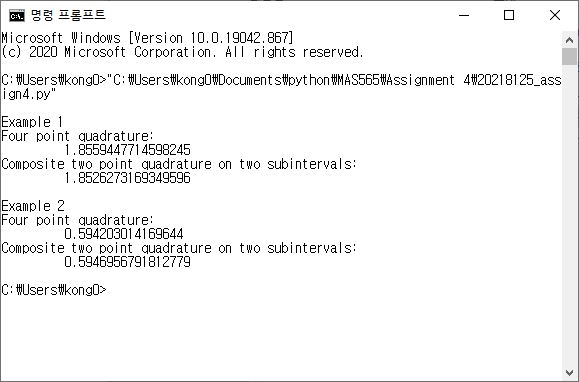
\includegraphics[width=0.8\linewidth]{console.JPG}
\end{center}
WolframAlpha tells us that the given integrals are approximately \begin{align*}
  I_1 &= \int_{-1}^1 e^{x^2} \ln(2-x)\, dx\, \approx\, 1.8557244913526205,\\
  I_2 &= \int_{1}^3 \frac{dx}{\sqrt{x^4+1}}\, \approx\, 0.59411342601921545.
\end{align*} We can see, in both cases, the four point Gaussian quadrature produces a better approximation of the integral than the two point composite Gaussian quadrature on two subintervals. 

\section*{Appendix}
As promised, we show that the Legendre polynomials $P_n(x)$ satisfy the recurrence relation \[
  P_{n+1}(x) = xP_n(x) - \frac{n^2}{4n^2-1}P_{n-1}(x), \quad n=1, 2, \cdots. 
  \]
  \begin{lemma}
    For any positive integer $n$, it holds that \[
      \ddx{n} x(x^2-1)^n = x\, \ddx{n}(x^2-1)^n + n\, \ddx{n-1}(x^2-1)^n.
    \]
  \end{lemma}\begin{proof}
    The general Leibniz rule states that for any $n$ times differentiable functions $f$ and $g$ it holds that \[
    (fg)^{(n)} = \sum_{k=0}^n \binom{n}{k} f^{(k)}g^{(n-k)}.  
    \] Applying the rule on $f(x) = x$ and $g(x) = (x^2-1)^n$, the derivatives of order higher than the second derivative of $f(x)$ is now zero, so the given equation immediately follows. 
  \end{proof}
  Now recall the formula (3.6.18) which states that \[
  P_n(x) = \frac{n!}{(2n)!} \ddx{n} (x^2 - 1)^n.
  \]
  \begin{lemma}
    It holds that \[
  xP_n(x) = \frac{n!}{(2n)!} \ddx{n-1} (x^2-1)^{n-1}\big((n+1)x^2 - (n-1)\big).
    \]
  \end{lemma} 
  \begin{proof}
     With the help of \textbf{Lemma 1} we get \begin{align*}
    xP_n(x) &= \frac{n!}{(2n)!}\cdot x\, \ddx{n} (x^2-1)^n  \\
            &= \frac{n!}{(2n)!}\left( \ddx{n} x(x^2-1)^n - n\, \ddx{n-1}(x^2-1)^n \right).
  \end{align*} Simple calculation leads to \begin{align*}
    \frac{(2n)!}{n!}\cdot xP_n(x) &= \ddx{n} x(x^2-1)^n - n\, \ddx{n-1}(x^2-1)^n \\
    &=  \ddx{n-1}\left(\ddx{}x(x^2-1)^n-n (x^2-1)^n \right) \\
    &=  \ddx{n-1}\left((x^2-1)^n+2nx^2(x^2-1)^{n-1}-n (x^2-1)^n \right) \\
    &=  \ddx{n-1}(x^2-1)^{n-1}\big((n+1)x^2+n-1\big)
  \end{align*} and the result follows. 
  \end{proof}
  \begin{lemma}
    The Legendre polynomials can also be represented as \[
    P_{n+1}(x) = \frac{(n+1)!}{(2n+1)!}\ddx{n-1} (x^2-1)^{n-1}\big((2n+1)x^2-1\big) .
    \]
  \end{lemma} \begin{proof}
    As we have \begin{align*}
      \ddx{2}(x^2-1)^{n+1} &= 2(n+1)\ddx{}\, x(x^2-1)^n \\
                           &= 2(n+1)(x^2-1)^n +2(n+1)x\cdot 2nx(x^2-1)^{n-1}\\
                           &= (2n+2)(x^2-1)^n + 4n(n+1)x^2(x^2-1)^{n-1} \\
                           &= (2n+2)(x^2-1)^{n-1}\big((2n+1)x^2-1\big)
    \end{align*} it follows that \begin{align*}
    P_{n+1}(x) &= \frac{(n+1)!}{(2n+2)!} \ddx{n-1}\left( \ddx{2} (x^2-1)^{n+1}  \right) \\
    &= \frac{(n+1)!}{(2n+1)!} \ddx{n-1}(x^2-1)^{n-1}\big((2n+1)x^2-1\big)
    \end{align*} which is exactly the claimed.
  \end{proof}
  Finally we are ready to show the following. 
  \begin{thm}
    The Legendre polynomials $P_n(x)$ satisfy the recurrence relation \[
  P_{n+1}(x) = xP_n(x) - \frac{n^2}{4n^2-1}P_{n-1}(x), \quad n=1, 2, \cdots. 
  \]
  \end{thm} \begin{proof}
    From \textbf{Lemma 3} and equation (3.6.18) in the textbook, we have \begin{align*}
      \frac{(2n+1)!}{(n+1)!} P_{n+1}(x) &= \ddx{n-1}(x^2-1)^{n-1}\big((2n+1)x^2 - 1\big)\, , \\
      \frac{(2n-2)!}{(n-1)!} P_{n-1}(x) &= \ddx{n-1}(x^2-1)^{n-1}
    \end{align*} Adding these two equations side by side and dividing both sides by $2n+1$ we get \[
      \ddx{n-1}\, x^2(x^2-1)^{n-1} = \frac{(2n)!}{(n+1)!}P_{n+1}(x) + \frac{(2n-2)!}{(n-1)!(2n+1)} P_{n-1}(x).
    \] For $n\geq 2$, by \textbf{Lemma 2} it follows that \begin{align*}
  \frac{(2n)!}{n!}\, xP_n(x)&= \ddx{n-1}(x^2-1)^{n-1}\big((n+1)x^2+n-1\big)\\
   &= (n+1)\left( \frac{(2n)!}{(n+1)!}P_{n+1}(x) + \frac{(2n-2)!}{(n-1)!(2n+1)} P_{n-1}(x) \right) + (n-1)\frac{(2n-2)!}{(n-1)!}P_{n-1}(x) \\
   &= \frac{(2n)!}{n!}P_{n+1}(x) + \left( \frac{(2n-2)!(n+1)}{(n-1)!(2n+1)} +{ \frac{(2n-2!)}{(n-2)!}} \right) P_{n-1}(x).
    \end{align*} Therefore \begin{align*}
      xP_n(x)&= P_{n+1}(x) + \left( \frac{n(n+1)}{2n(2n-1)(2n+1)}+\frac{n(n-1)}{2n(2n-1)}\right) P_{n-1}(x) \\
      &= P_{n+1}(x) + \frac{n^2}{(2n-1)(2n+1)} P_{n-1}(x)
    \end{align*} hence the given recurrence relation. By noting that $P_2(x) = x^2-\dfrac{1}{3}$, $P_1(x) =x$, and $P_0(x)= 1$ we see that the recurrence relation also holds for $n=1$.  
  \end{proof}
\end{document}